%%%%%%%%%%%%%%%%%%%%%%%%%%%%%%%%%%%%%%%%%%%%%%%%%%%%%%%%%%%%%%%%%%%%%%%%%%%%%%%
% PLANTILLA DE REPORTE / WALKTHROUGH DE CIBERSEGURIDAD
% Autor: (Tu nombre, 15 años de experiencia ;) )
%%%%%%%%%%%%%%%%%%%%%%%%%%%%%%%%%%%%%%%%%%%%%%%%%%%%%%%%%%%%%%%%%%%%%%%%%%%%%%%

\documentclass[12pt,a4paper]{report}

%==============================================================================
% PAQUETES Y CONFIGURACIONES BÁSICAS
%==============================================================================
\usepackage[spanish]{babel}        % Idioma en español
\usepackage[utf8]{inputenc}        % Acentos y caracteres en UTF-8
\usepackage[T1]{fontenc}           % Codificación de fuente
\usepackage{geometry}              % Control de márgenes
\usepackage{graphicx}              % Para incluir imágenes
\usepackage{float}                 % Control de posiciones de figuras
\usepackage{fancyhdr}              % Encabezados y pies de página profesionales
\usepackage{titlesec}              % Control de títulos
\usepackage{minted}                % Para resaltar código con colores (necesita -shell-escape)
\usepackage{hyperref}              % Hipervínculos y referencias clicables
\usepackage{tocloft}               % Personalización del índice

%==============================================================================
% CONFIGURACIONES DE PÁGINA
%==============================================================================
\geometry{
    left=2.5cm,
    right=2.5cm,
    top=3cm,
    bottom=3cm
}

%==============================================================================
% PERSONALIZACIÓN DE TÍTULOS
%==============================================================================
\titleformat{\chapter}[hang]
  {\normalfont\huge\bfseries}
  {}
  {0pt}
  {\thechapter.\ }

%==============================================================================
% CONFIGURACIÓN DE HIPERVÍNCULOS
%==============================================================================
\hypersetup{
    colorlinks=true,         % Activa colores en lugar de cuadros
    linkcolor=red,           % Color de los enlaces internos (como el índice)
    urlcolor=blue,           % Color de los hipervínculos a internet
    linkbordercolor={0 0 0}, % Desactiva el color del borde (cuadro rojo)
    urlbordercolor={0 0 0},  % Desactiva el color del borde en URLs (cuadro azul)
}

%==============================================================================
% VARIABLES (MODIFICAR AQUÍ SEGÚN TU PROYECTO)
%==============================================================================
\newcommand{\machineName}{Test}
\newcommand{\machineURL}{https://test.com} 
\newcommand{\platformName}{Hack The HackTheBox} % (HackTheBox, TryHackMe, etc.)
\newcommand{\authorName}{Franco Javier Lazzarini} 
\newcommand{\myLogo}{images/my_logo.png}          % Logo personal (reemplazar archivo)
\newcommand{\platformLogo}{images/platform_logo.png} % Logo de la plataforma (reemplazar archivo)
\newcommand{\reportDate}{\today}                  % Fecha (puedes usar una fija si prefieres)

%==============================================================================
% CONFIGURACIÓN DE ENCABEZADOS Y PIES
%==============================================================================
\fancypagestyle{general}{
  \fancyhf{} % Limpia encabezado y pie
  \renewcommand{\headrulewidth}{0.4pt}
  \lhead{\includegraphics[height=1.0cm]{\myLogo}}
  \rhead{\includegraphics[height=1.0cm]{\platformLogo}}
  \cfoot{\thepage}
}

% Redefinimos el estilo 'plain' (usado en páginas de capítulo) para que use 'general'
\makeatletter
\let\ps@plain\ps@general
\makeatother

%==============================================================================
% INICIO DEL DOCUMENTO
%==============================================================================
\begin{document}

%==============================================================================
% PORTADA (SIN NUMERACIÓN)
%==============================================================================
\begin{titlepage}
    \centering
    \vspace*{3cm}

    {\huge \textbf{Reporte de la Máquina \machineName}\\[1em]}
    
    {\Large \platformName}\\[1em]
    
    \vfill
    
    \textbf{Autor:} \authorName \\
    \textbf{Fecha:} \reportDate \\
    
    \vspace*{2cm}
    
    \includegraphics[width=0.4\textwidth]{\myLogo}
    \hspace{0.5cm}
    \includegraphics[width=0.4\textwidth]{\platformLogo}
    
    \vfill
    \thispagestyle{empty} % Sin encabezado/pie ni número en la portada
\end{titlepage}

%==============================================================================
% ÍNDICE (PÁGINA 1)
%==============================================================================
\pagestyle{general}   % Aplica el estilo fancy definido
\pagenumbering{arabic}% Numeración arábiga
\setcounter{page}{1}  % Arrancamos en la página 1

\tableofcontents
\clearpage

%==============================================================================
% 1. INFORMACIÓN GENERAL
%==============================================================================
\chapter{Información General}

\section{Descripción}
\textbf{Máquina:} \machineName

Plataforma: \platformName

URL de la máquina: \href{\machineURL}{\machineURL}

\section{Objetivos}
\begin{itemize}
    \item Objetivo principal: \textit{Obtener acceso a la máquina, enumerar vulnerabilidades y, en última instancia, escalar privilegios}.
    \item Objetivos secundarios: \textit{Aprender nuevas técnicas de enumeración, probar herramientas específicas, etc.}
\end{itemize}

%==============================================================================
% 2. RECONOCIMIENTO
%==============================================================================
\chapter{Fase de Reconocimiento}

\section{Enumeración de Servicios}
Aquí puedes detallar qué puertos, servicios o versiones encontraste. Por ejemplo:
\begin{minted}[frame=lines, framesep=2mm, fontsize=\small, bgcolor=gray!10]{bash}
nmap -sC -sV -oN nmap_inicial.txt 10.10.10.X
# Resultados relevantes:
# PORT   STATE SERVICE VERSION
# 80/tcp open  http    Apache httpd 2.4.41
\end{minted}

Puedes incluir capturas de pantalla:

\begin{figure}[H]
    \centering
    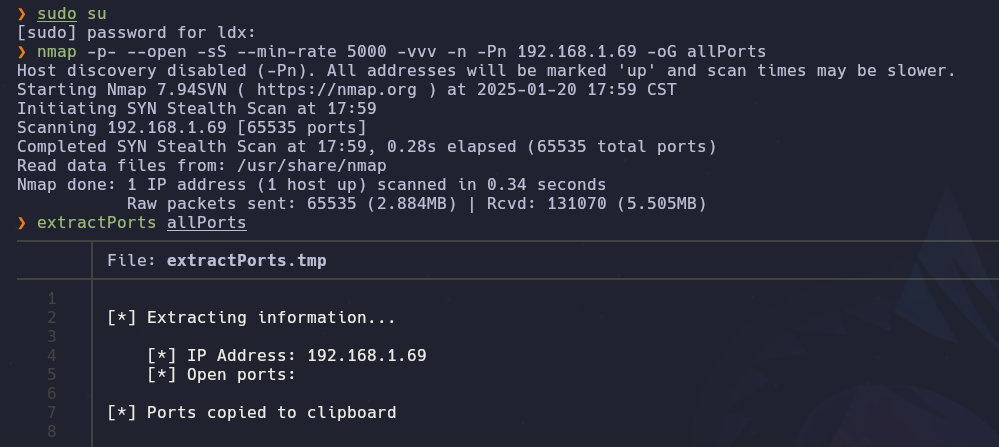
\includegraphics[width=0.75\linewidth]{images/placeholder_nmap.png}
    \caption{Resultado del escaneo Nmap}
    \label{fig:nmap-scan}
\end{figure}

\section{Enumeración Web}
Texto de ejemplo explicando cómo enumeraste la aplicación web, carpetas, subdominios, etc.

%==============================================================================
% 3. EXPLOTACIÓN
%==============================================================================
\chapter{Fase de Explotación}

\section{Vector de Ataque Principal}
Explica la vulnerabilidad encontrada (por ejemplo, inyección SQL, RCE, etc.).  
Ejemplo de código usado o payload:
\begin{minted}[frame=lines, framesep=2mm, fontsize=\small, bgcolor=gray!10]{bash}
# Ejemplo de exploit en Python
python exploit.py --target 10.10.10.X --port 80
\end{minted}

\section{Obtención de Acceso (Shell Inicial)}
Descripción de cómo conseguiste la primera shell en el sistema, con capturas de pantalla si es necesario.

%==============================================================================
% 4. ESCALADA DE PRIVILEGIOS
%==============================================================================
\chapter{Escalada de Privilegios}

\section{Enumeración de Sistema}
Explica las herramientas o comandos que usaste (p.ej. LinPEAS, WinPEAS, etc.).

\section{Explotación de la Vulnerabilidad Interna}
Describe la técnica de escalada de privilegios, adjunta cualquier script, etc.

\section{Acceso Como ROOT/Administrator}
Demuestra finalmente el acceso con máximos privilegios.

\begin{figure}[H]
    \centering
    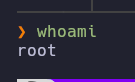
\includegraphics[width=0.7\linewidth]{images/placeholder_root.png}
    \caption{Shell con privilegios elevados}
    \label{fig:root-shell}
\end{figure}

%==============================================================================
% 5. RECOMENDACIONES DE MITIGACIÓN
%==============================================================================
\chapter{Recomendaciones}

\section{Vulnerabilidad X}
- Explica la causa de la vulnerabilidad y posibles soluciones.

\section{Buenas Prácticas Adicionales}
- Enumera mejores prácticas generales de seguridad (segmentación de red, hardening de servicios, etc.).

%==============================================================================
% 6. CONCLUSIONES
%==============================================================================
\chapter{Conclusiones}

Resumen final de los hallazgos, reflexión sobre el proceso y aprendizaje adquirido.

\section{Observaciones Personales}
Agrega notas finales, lecciones aprendidas, etc.

%==============================================================================
% FIN DEL DOCUMENTO
%==============================================================================
\end{document}
